\chapter{Detalles de Implementación y Experimentos}\label{chapter:implementation}

En este capítulo se presentan las pruebas que se hicieron para evaluar
 el desempeño de los modelos. Para estas pruebas se utilizaron datos...

\begin{table}[ht]
    \centering
    \caption{Resultados de Clustering}
    \begin{tabular}{lccc}
        \toprule
        \textbf{Método} & \textbf{Silhouette} & \textbf{Calinski Harabaz} & \textbf{Davies Bouldin} \\
        \midrule
        Agglomerative Clustering & 0.2236 & 186.1952 & 1.4984 \\
        DBSCAN & 0.4641 & 25.136239627069884 & 1.6503 \\
        K-Mean & - & - &
        \bottomrule
    \end{tabular}
\end{table}

A continuación se presentan las gráficas de los dos modelos implementados en el estudio: Isolation Forest y One-Class SVM. Para mejorar la interpretación de estos resultados, se han utilizado herramientas de reducción de dimensionalidad como PCA (Análisis de Componentes Principales) y t-SNE (t-Distributed Stochastic Neighbor Embedding).\\

\begin{itemize}
	\item {\textbf{Análisis de Componentes Principales (PCA):}}El PCA es una técnica fundamental en el análisis exploratorio de datos y en la reducción de la dimensionalidad. Funciona transformando un conjunto de variables posiblemente correlacionadas en un conjunto más pequeño de variables linealmente no correlacionadas llamadas componentes principales. Estos componentes capturan la mayor parte de la variabilidad presente en los datos originales. Al aplicar PCA a nuestros datos antes de visualizar los resultados de los modelos de Isolation Forest y One-Class SVM, esperamos observar cómo se agrupan o dispersan los datos en un espacio de menor dimensión. Esto puede revelar patrones de agrupación o anomalías que no son tan evidentes en el espacio original de alta dimensión.
	
	\item {\textbf{t-Distributed Stochastic Neighbor Embedding (t-SNE):}} 
t-SNE es una técnica avanzada de reducción de dimensionalidad que se utiliza principalmente para la visualización de datos de alta dimensionalidad en espacios de menor dimensión (generalmente 2D o 3D). A diferencia de PCA, t-SNE no se basa en proyecciones lineales, sino que se centra en preservar las distancias entre puntos en el espacio original, especialmente las distancias locales.
\end{itemize}


\begin{figure}[ht]
  \centering
  \begin{minipage}[b]{0.45\linewidth}
    \centering
    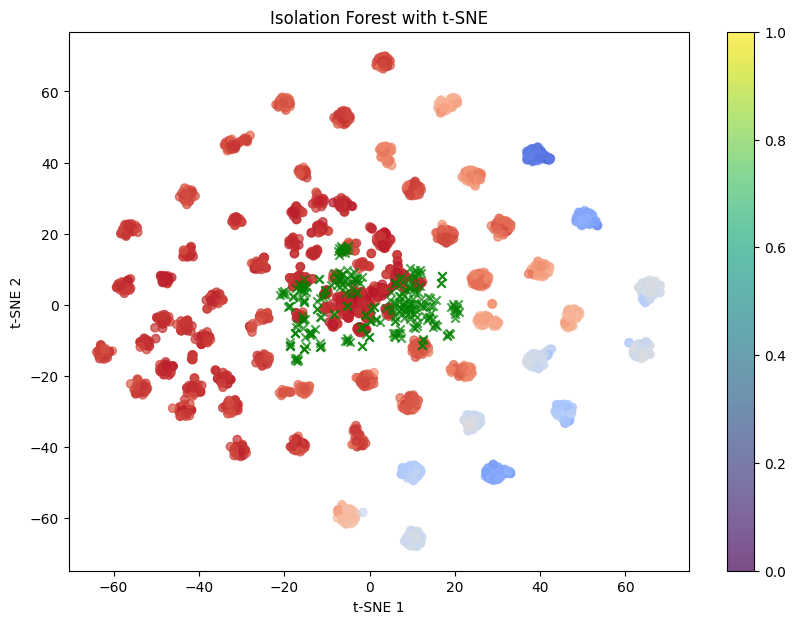
\includegraphics[width=\linewidth]{Graphics/isolation_forest_Tsne.png} % Nombre de la primera imagen
    %\caption{Primera imagen}
  \end{minipage}
  \hspace{0.5cm} % Espacio horizontal entre las dos imágenes
  \begin{minipage}[b]{0.45\linewidth}
    \centering
    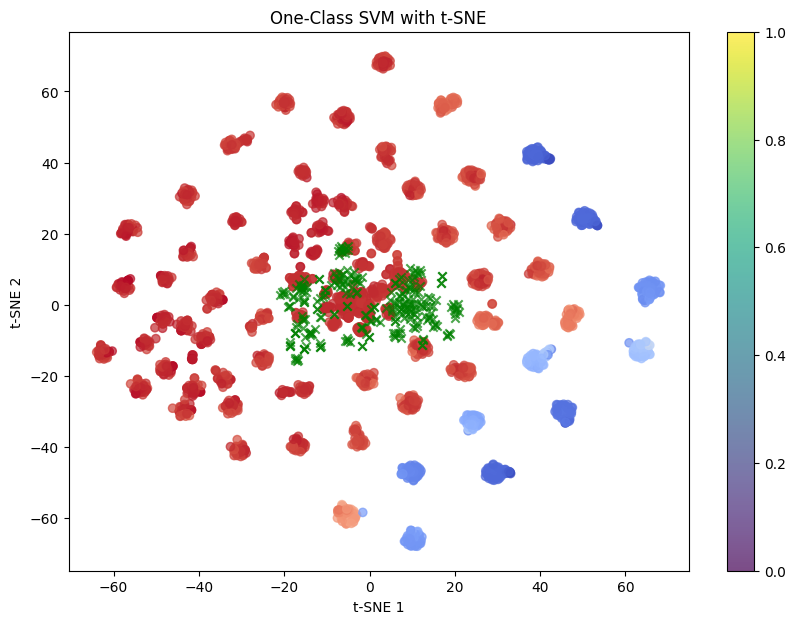
\includegraphics[width=\linewidth]{Graphics/one_class_svm_Tsne.png} % Nombre de la segunda imagen
    %\caption{Segunda imagen}
  \end{minipage}
\end{figure}


\begin{figure}[ht]
  \centering
  \begin{minipage}[b]{0.45\linewidth}
    \centering
    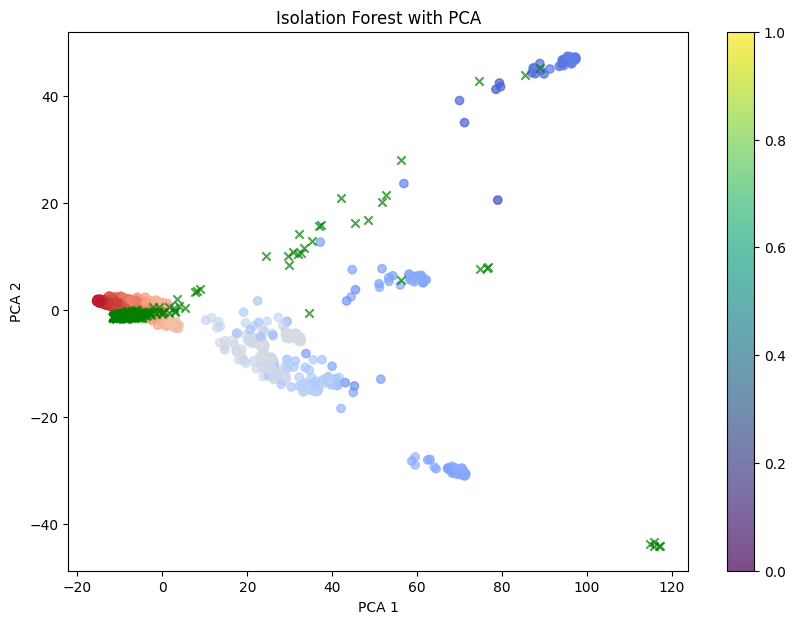
\includegraphics[width=\linewidth]{Graphics/isolation_forest_PCA.png} % Nombre de la primera imagen
    %\caption{Primera imagen}
  \end{minipage}
  \hspace{0.5cm} % Espacio horizontal entre las dos imágenes
  \begin{minipage}[b]{0.45\linewidth}
    \centering
    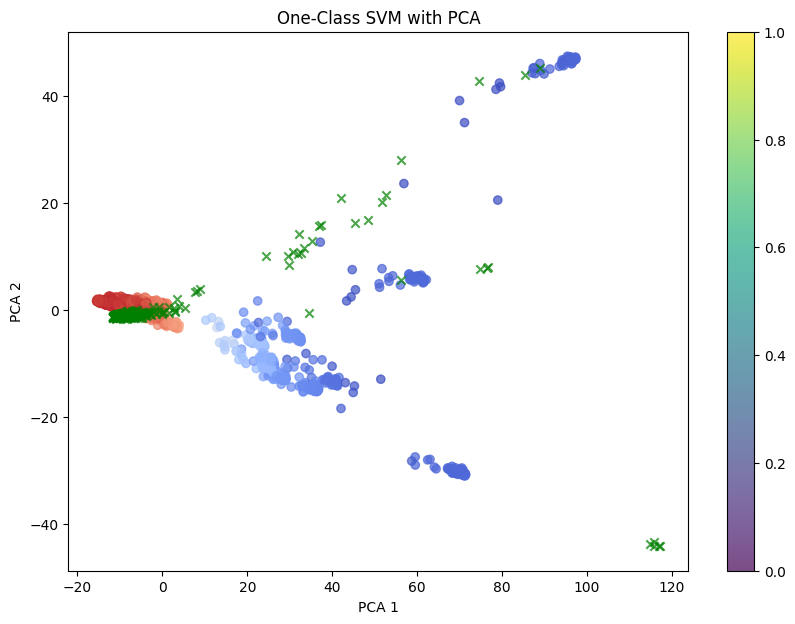
\includegraphics[width=\linewidth]{Graphics/one_class_svm_PCA.png} % Nombre de la segunda imagen
    %\caption{Segunda imagen}
  \end{minipage}
\end{figure}


\begin{table}[ht]
\centering
\begin{tabular}{lcc}
\toprule
\textbf{Modelo} & \textbf{Error en entrenamiento} & \textbf{Error en prueba} \\
\midrule
Isolation Forest & 388/3880 & 74/712 \\
One-Class SVM & 758/3880 & 147/712 \\
\bottomrule
\end{tabular}
\caption{Errores de Isolation Forest y One-Class SVM}
\label{tab:resultados}
\end{table}

Los resultados indican que tanto Isolation Forest como One-Class SVM muestran promesa en la identificación de anomalías dentro del espacio de vectores de similitud de código. Isolation Forest logró tasas de error más bajas en comparación con One-Class SVM en ambos conjuntos de entrenamiento y prueba, lo que sugiere que puede ser más efectivo para aislar muestras de código disímiles. Sin embargo, estos hallazgos son preliminares debido a problemas continuos con la extracción precisa del árbol de sintaxis abstracta. Por lo tanto, estas tasas de error aún no representan completamente el rendimiento final de los modelos.\\

Es importante destacar que las tasas de error reportadas están influenciadas por la calidad de la extracción del AST. ASTs inexactos o incompletos pueden llevar a una representación errónea de las estructuras de código, afectando así la evaluación del rendimiento de los algoritmos de detección de anomalías. Abordar estos problemas es crucial para obtener resultados más confiables.